\basicheader
\usepackage{ifthen,etoolbox}
\usepackage[ngerman]{babel}
\usepackage{colortbl}
\usepackage{longtable}

\setlength{\LTpost}{\medskipamount}

\usepackage[sfdefault,tabular,scaled=.9]{FiraSans}
\usepackage[lining,scaled=.9]{FiraMono}
\usepackage[mathrm=sym]{unicode-math}
\usepackage[Scale=.9]{firamath-otf}
\usepackage{luatexbase}
\usepackage{microtype}
\usepackage[hang,symbol,multiple]{footmisc}
\usepackage{tikz}

\renewcommand{\footnotemargin}{1em}

\input graphdrawing.tex

\input translation-\ifcsdef{TemplateLanguage}{\TemplateLanguage}{de}.tex

\newlength{\myoddoffset}
\setlength{\myoddoffset}{\marginparwidth + \marginparsep + \marginparsep}
\fancyheadoffset[roh,reh]{\myoddoffset}

\def\logo{
\begin{tikzpicture}
    \begin{scope}[yshift=.75cm]
        \node[white!40!black, rotate=16.125, anchor=west, align=left] at (15:2.25cm)
        {\mbox{}\\[.6ex]{\bfseries\contestname\quad}\\\tTask:\enspace\bfseries\taskname\quad\\[-.8ex]};
    \end{scope}

    \path (current bounding box.north east);
    \pgfgetlastxy{\XCoord}{\YCoord};
    \pgfmathsetmacro{\bndx}{max(215, \XCoord)};
    \pgfmathsetmacro{\bndy}{max(200, \YCoord)};

    \clip (0,0) rectangle (\bndx pt,\bndy pt);
    \node[anchor=south west] (pic) at (0, 0) {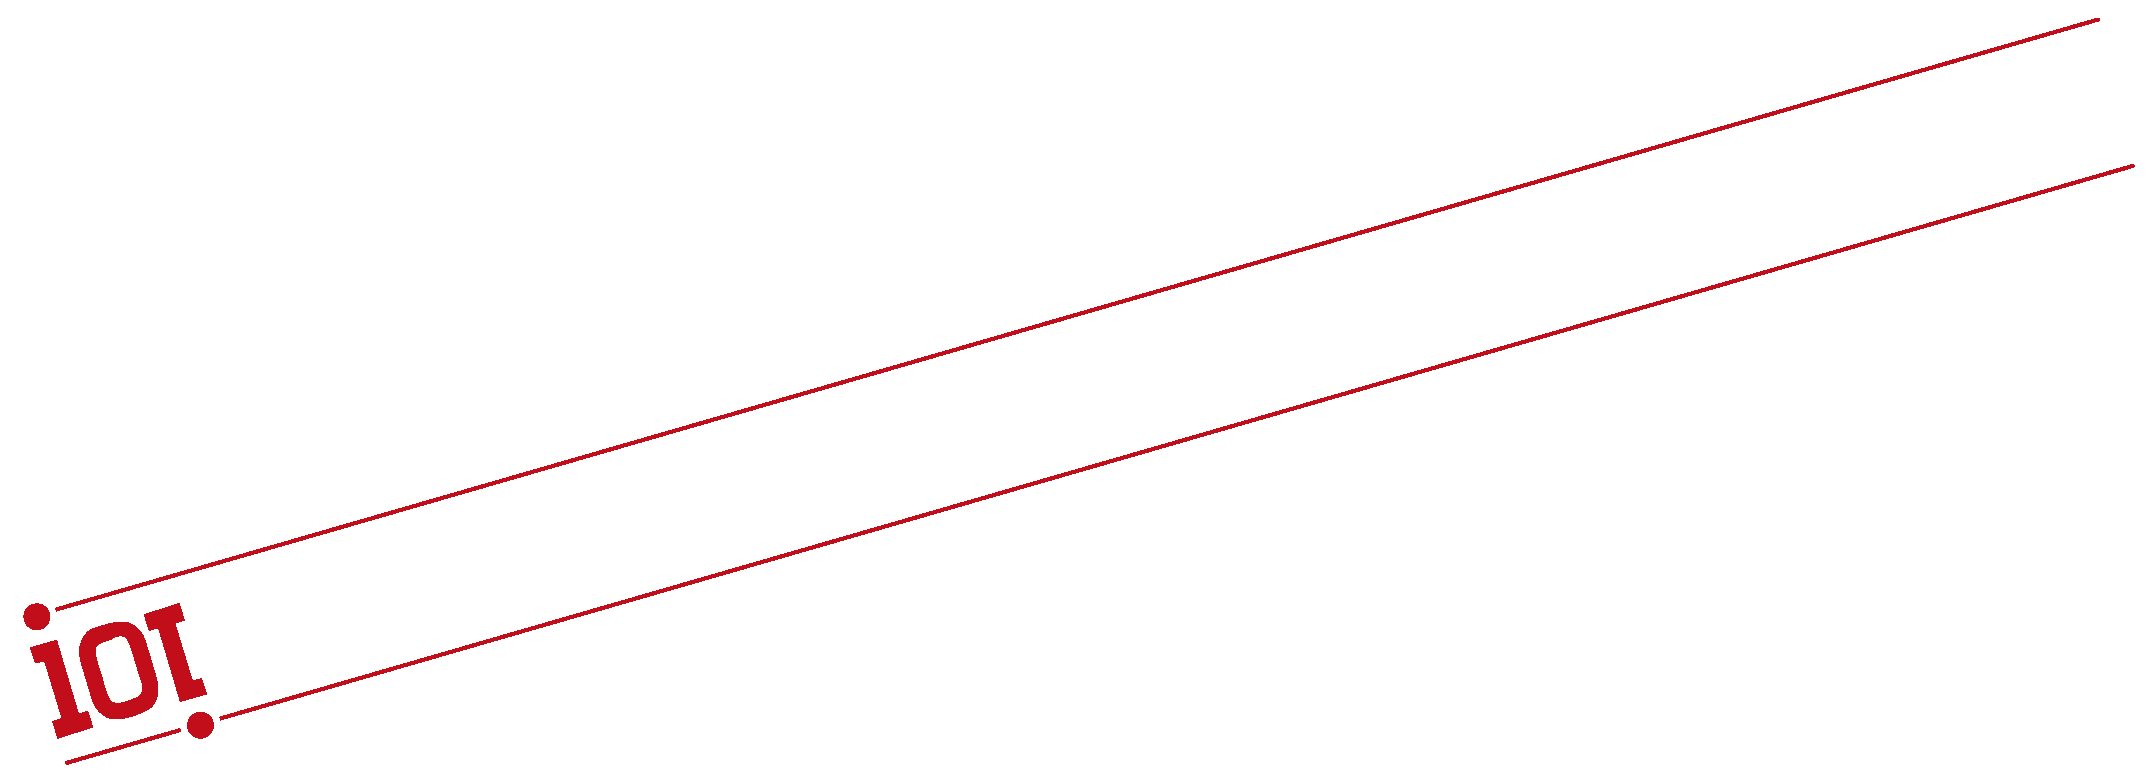
\includegraphics[scale=.55]{logo.eps}};
\end{tikzpicture}
}

%\rhead{\vbox to \headh{\vbox to 0pt{\vskip-2in\hbox to 0pt{\hskip\hsize\hskip-1.5in\includegraphics{\barpdf}}}\quad\null}}
\rhead{\vbox to \headh{\vbox to 0pt{\vskip-2in{\logo}}\quad\null}}

\lhead{}

\makeatletter
\def\sthelper#1#2{{\sffamily\bfseries \tSubtask\ #1 ($\symbf{#2}$ \ifnum#2=1\tPoint\else\tPoints\fi).\enspace}}
\newcount\stcount
\stcount=0
\def\st#1{\setbox0=\hbox{\sthelper{9}{99}}\global\advance\stcount by 1 \par\ifdim\lastskip<\smallskipamount\removelastskip\smallskip\fi\noindent\hangindent=\wd0 \hangafter=1 \hbox to \wd0{\sthelper{\the\stcount}{#1}\hss}\ignorespaces}
\def\subtask{\count1=\stcount \advance\count1 by 1 \st{\subtaskpoints{\the\count1}}}
\def\currconstraint#1{\scopedconstraint{\the\stcount}{#1}}
\def\currconstraints{\@ifstar{\currconstraint{@ll*}}{\currconstraint{@ll}}}
\def\currconstraintupper#1{\scopedconstraintupper{\the\stcount}{#1}}
\def\currconstraintlower#1{\scopedconstraintlower{\the\stcount}{#1}}
\def\currconstraintvalue#1{\scopedconstraintvalue{\the\stcount}{#1}}

\begingroup
\catcode`\ǁ=4
\catcode`\& =\active%
\gdef\@ctivateAMP{\def&{ǁǁ}}
\endgroup
\newenvironment{interactiontable}{\begingroup%
\catcode`\& =\active%
\@ctivateAMP%
\par\medskip%
\begin{tabular}{>{\cellcolor[gray]{.9}}p{3.5cm}@{\hskip0pt}p{.52cm}@{\hskip0pt}>{\cellcolor[gray]{.9}}p{3cm}@{\hskip0pt}p{.52cm}@{\hskip0pt}>{\cellcolor[gray]{.9}\sffamily\hangindent=1.25em\hangafter=1\raggedright\arraybackslash}p{7.55cm}}
\hline
\multicolumn{1}{|c}{\cellcolor{white}\sffamily\tProgram}&&\multicolumn{1}{c}{\sffamily \tReturn}&&\multicolumn{1}{c|}{\sffamily\tExplanation}\\\hline
\noalign{\smallskip}%
}{\end{tabular}\endgroup\par\medskip}

\def\myc@ption#1#2#3{\noalign{\bfseries\large #3}}
\def\showcases{\removelastskip\par\bigskip\begingroup%
% This is evil: we hijack LT@makecaption to force longtable to place the heading
% same page as the table...
\let\LT@makecaption=\myc@ption
\begingroup%
\microtypesetup{activate=false}%
\testcasetable%
\endgroup%
\endgroup}
\def\showlimits{\sheading{\tLimits}%
\tTime: \timelimit\\
\tMemory: \memlimit}

% Feedback Section
\def\feedbackheading{\sheading{\tFeedback}}
\def\nofeedback{\feedbackheading \tNofeedback}
\def\partialfeedback{\feedbackheading \tPartialfeedback}
\def\fullfeedback{\feedbackheading\def\feedbackmode{\ifrestricted\emph{restricted feedback}\else\emph{full feedback}\fi} \tFullfeedbackGeneral\
\ifrestricted
\tRestrictedfeedbackPrecise
\else
\tFullfeedbackPrecise
\fi}
\def\tokenfeedback{\feedbackheading \tTokenFeedback

\ifrestricted
\tTokenRestrictedFeedback
\fi}
\let\dummyfeedack=\relax
\def\showfeedback{\csname\feedback feedback\endcsname}

% Scoring Section
\def\scoringheading{\sheading{\tScoring}}
\def\IOIXIIIscoring{\scoringheading \tScoringFromIOIXIII}
\def\IOIXVIIscoring{\scoringheading \tScoringFromIOIXVII}
\def\IOIXscoring   {\scoringheading \tScoringFromIOIX}
\def\showscoring{\csname\scoring scoring\endcsname}

% ---

\def\standardpart{\showcases\showlimits\showfeedback\showscoring}
\makeatother

\def\flushsubtasks{\global\stcount=\numsubtasks}

\AtEndDocument{\ifnum\stcount=\numsubtasks\else\PackageError{lg-template}{Not all subtasks are contained in the task statement!\MessageBreak You should call \protect\subtask\space (or \protect\st) precisely as often as there are subtasks, not counting the public one. If for some reason you do not want to do this, you can call \protect\flushsubtasks\space after all calls to \protect\subtask\space and \protect\st}{You should call \protect\subtask\space (or \protect\st) precisely as often as there are subtasks, not counting the public one. If for some reason you do not want to do this, you can call \protect\flushsubtasks\space after all calls to \protect\subtask\space and \protect\st}\fi}
